%%
%% Copyright 2007, 2008, 2009 Elsevier Ltd
%%
%% This file is part of the 'Elsarticle Bundle'.
%% ---------------------------------------------
%%
%% It may be distributed under the conditions of the LaTeX Project Public
%% License, either version 1.2 of this license or (at your option) any
%% later version.  The latest version of this license is in
%%    http://www.latex-project.org/lppl.txt
%% and version 1.2 or later is part of all distributions of LaTeX
%% version 1999/12/01 or later.
%%
%% The list of all files belonging to the 'Elsarticle Bundle' is
%% given in the file `manifest.txt'.
%%

%% Template article for Elsevier's document class `elsarticle'
%% with numbered style bibliographic references
%% SP 2008/03/01

\documentclass[preprint,12pt, a4paper]{elsarticle}

%% Use the option review to obtain double line spacing
%% \documentclass[authoryear,preprint,review,12pt]{elsarticle}

%% For including figures, graphicx.sty has been loaded in
%% elsarticle.cls. If you prefer to use the old commands
%% please give \usepackage{epsfig}

%% The amssymb package provides various useful mathematical symbols
\usepackage{amssymb}
\usepackage{hyperref}
\usepackage{svg}
\setlength{\parindent}{0pt}
%% The amsthm package provides extended theorem environments
%% \usepackage{amsthm}

%% The lineno packages adds line numbers. Start line numbering with
%% \begin{linenumbers}, end it with \end{linenumbers}. Or switch it on
%% for the whole article with \linenumbers.
%\usepackage{lineno}

\journal{SoftwareX}

\begin{document}
\renewcommand{\labelenumii}{\arabic{enumi}.\arabic{enumii}}

\begin{frontmatter}
%% Title, authors and addresses

%% use the tnoteref command within \title for footnotes;
%% use the tnotetext command for theassociated footnote;
%% use the fnref command within \author or \address for footnotes;
%% use the fntext command for theassociated footnote;
%% use the corref command within \author for corresponding author footnotes;
%% use the cortext command for theassociated footnote;
%% use the ead command for the email address,
%% and the form \ead[url] for the home page:
%% \title{Title\tnoteref{label1}}
%% \tnotetext[label1]{}
%% \author{Name\corref{cor1}\fnref{label2}}
%% \ead{email address}
%% \ead[url]{home page}
%% \fntext[label2]{}
%% \cortext[cor1]{}
%% \address{Address\fnref{label3}}
%% \fntext[label3]{}

\title{Foruster: Live system data extraction}

%% use optional labels to link authors explicitly to addresses:
%% \author[label1,label2]{}
%% \address[label1]{}
%% \address[label2]{}

\author[label1]{Marcos Jesús Sequera Fernández}
\author[label2]{A. Author2}
\address[label1]{marcosjesus@unex.es}
\address[label2]{Author2's affiliation, address, email}

\begin{abstract}
%% Text of abstract
Foruster is a cross-platform desktop application, developed in Rust, for live-system forensic analysis. Unlike traditional tools that require system shutdown, Foruster is designed to identify and catalog files of interest on active storage volumes. Its user interface, built with the Slint framework, guides the analyst through the selection of devices, the configuration of search profiles, and the real-time visualization of results. The software features heuristic detection of anomalies, such as deceptive file extensions, and ensures the integrity of findings through cryptographic hashing, optimizing the digital forensic investigation process.
\end{abstract}

\begin{keyword}
%% keywords here, in the form: keyword \sep keyword
live-system forensics \sep forensic software \sep data extraction \sep Rust \sep digital security \sep incident response

%% PACS codes here, in the form: \PACS code \sep code

%% MSC codes here, in the form: \MSC code \sep code
%% or \MSC[2008] code \sep code (2000 is the default)

\end{keyword}

\end{frontmatter}

%\linenumbers

\section*{Metadata}
\label{}

\begin{table}[!h]
\begin{tabular}{|l|p{6.5cm}|p{6.5cm}|}
\hline
\textbf{Nr.} & \textbf{Code metadata description} & \textbf{Metadata} \\
\hline
C1 & Current code version & 1.0.0 \\
\hline
C2 & Permanent link to code/repository used for this code version & \url{https://github.com/m4rz3r0/foruster} \\
\hline
C3  & Permanent link to Reproducible Capsule & –\\
\hline
C4 & Legal Code License & GPLv3 \\
\hline
C5 & Code versioning system used & git \\
\hline
C6 & Software code languages, tools, and services used & Rust, Slint  \\
\hline
C7 & Compilation requirements, operating environments \& dependencies & Rust 1.89 \\
\hline
C8 & If available Link to developer documentation/manual & - \\
\hline
C9 & Support email for questions & marcosjesus@unex.es \\
\hline
\end{tabular}
\caption{Code metadata (mandatory)}
\label{codeMetadata}
\end{table}

\section{Motivation and significance}
El análisis forense digital tradicional, basado en la adquisición de imágenes de sistemas apagados, presenta desafíos significativos como la pérdida de evidencia volátil y la complejidad para acceder a volúmenes cifrados. Foruster aborda este problema al proporcionar una herramienta para el análisis de sistemas de archivos en vivo. Su importancia radica en la capacidad de realizar un triaje rápido y no invasivo, permitiendo el acceso a datos en volúmenes cifrados desbloqueados (como BitLocker o LUKS) y preservando el estado operativo del sistema.

El software contribuye al proceso de descubrimiento forense al facilitar el estudio de la evidencia volátil y optimizar la fase inicial de una investigación. En su uso práctico, el analista ejecuta la aplicación en el sistema objetivo, selecciona dispositivos y perfiles de búsqueda a través de una interfaz gráfica, y recibe resultados en tiempo real, incluyendo la detección de anomalías heurísticas.

\section{Descripción del Software}

Foruster es una aplicación de escritorio multiplataforma, desarrollada en \textbf{Rust}, diseñada para el análisis forense de sistemas en vivo. A diferencia de las herramientas tradicionales que requieren apagar el sistema, Foruster está específicamente diseñado para identificar y catalogar archivos de interés en volúmenes de almacenamiento activos. Su interfaz de usuario se construye con el framework \textbf{Slint}, lo que resulta en una aplicación nativa que guía al analista a través del proceso de selección de dispositivos, configuración de perfiles y una visualización de resultados en tiempo real.

\subsection{Arquitectura Modular y Pila Tecnológica}

El diseño de Foruster se basa en una arquitectura modular implementada mediante un \textit{workspace} de Rust, separando la funcionalidad en capas lógicas a través de diferentes \textit{crates} para optimizar la mantenibilidad y el rendimiento (ver Figura~\ref{fig:arquitectura}).

En la base se encuentra el \textit{crate} \texttt{foruster-storage}, que gestiona la complejidad de la interacción con el sistema operativo. Esta capa encapsula las diferencias entre plataformas para detectar y enumerar los dispositivos de almacenamiento. Para la interacción con el almacenamiento en \textbf{Windows}, Foruster utiliza directamente las APIs nativas de Win32 (a través del \textit{crate} \texttt{windows}), lo que le permite consultar volúmenes lógicos (\texttt{FindFirstVolumeW}) y discos físicos mediante el envío de códigos de control de E/S (\texttt{DeviceIoControl} sobre rutas como \texttt{$\backslash$$\backslash$.$\backslash$PhysicalDriveX}). En sistemas \textbf{Linux}, el \textit{crate} interactúa con los sistemas de archivos virtuales \texttt{/sys/block} y \texttt{/proc/self/mountinfo} para construir el mapa de discos y particiones.

La lógica de negocio se implementa en los \textit{crates} \texttt{analysis} y \texttt{profiling}. El motor de análisis se ejecuta de forma concurrente sobre el \textit{runtime} asíncrono \textbf{Tokio}, utilizando el \textit{crate} \texttt{async-walkdir} para una exploración eficiente de los sistemas de archivos. Este motor es el responsable de aplicar las reglas de los "Perfiles" de búsqueda (definidos en \texttt{profiling}), que son colecciones de criterios basados en categorías de archivos, tipos MIME o extensiones específicas.

Finalmente, la capa \texttt{api} actúa como un puente intermedio, transformando las estructuras de datos del \textit{backend} en interfaces seguras y fáciles de consumir por la interfaz gráfica (\texttt{desktop}).

\begin{figure}[h!]
    \centering
    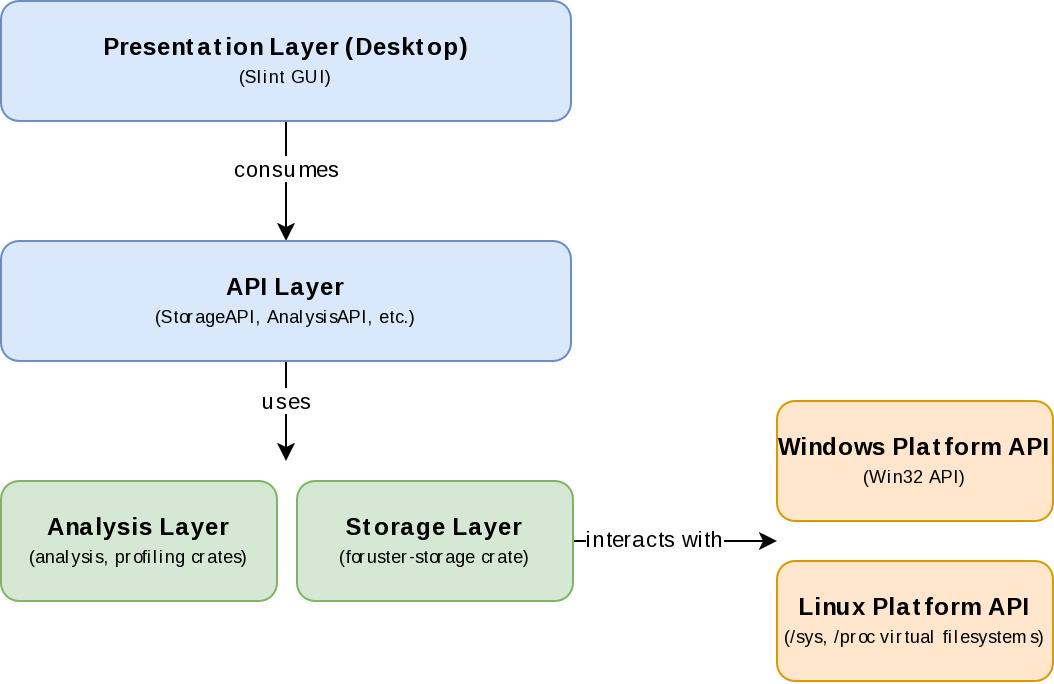
\includegraphics[width=0.8\textwidth]{resources/foruster_architecture.jpg}
    \caption{Diagrama de la arquitectura de Foruster, mostrando sus capas modulares desde la interfaz de usuario hasta la interacción con el sistema operativo.}
    \label{fig:arquitectura}
\end{figure}

\subsection{Admisibilidad Probatoria y Cumplimiento de la Cadena de Custodia}

La correcta extracción de evidencia digital basada en ficheros requiere un enfoque metodológico que garantice su integridad y autenticidad, un principio fundamental para su admisibilidad probatoria. La norma ISO/IEC 27037 proporciona directrices clave en este ámbito. En escenarios de análisis en vivo ("trabajo en caliente"), la metodología debe minimizar la huella sobre el sistema, preservar los metadatos de los archivos y asegurar la trazabilidad mediante una cadena de custodia robusta. Foruster ha sido diseñado para operar dentro de este riguroso marco, estructurando sus funcionalidades en torno a las fases forenses de identificación, adquisición, preservación y presentación.

\subsubsection{Fase de Identificación y Adquisición}

Esta fase se centra en la localización y recolección de la evidencia potencial. Foruster aborda este punto permitiendo una selección reproducible del ámbito de análisis, donde el investigador define los dispositivos de almacenamiento y los perfiles de búsqueda. El motor de análisis (analysis::walker) opera sobre la capa del sistema de archivos, lo que minimiza la interacción directa con el hardware y reduce la huella en el sistema. Esta aproximación permite la adquisición de datos de volúmenes cifrados (BitLocker, LUKS) que se encuentren montados, un escenario común en sistemas activos. Además, Foruster implementa heurísticas para la identificación de anomalías, como la discrepancia entre el tipo de archivo real (verificado mediante "magic numbers" con el crate file-format) y su extensión, descubriendo así evidencia que podría haber sido ofuscada intencionadamente.

\subsubsection{Fase de Preservación y Aportación}

Para garantizar que la evidencia no sea alterada ni contaminada, la fase de preservación es crítica. Foruster asegura la integridad de cada archivo identificado mediante la generación de múltiples huellas criptográficas. Para cada fichero relevante, el software calcula sus hashes MD5, SHA-256 y BLAKE3. Este conjunto de hashes actúa como una firma digital única del estado del archivo en el momento exacto de la adquisición. Este proceso es fundamental para la aportación de la prueba, ya que establece una cadena de custodia auditable. Cualquier verificación posterior puede recalcular estos hashes para confirmar que la evidencia presentada es una copia exacta de la original.

\subsubsection{Fase de Presentación}

La presentación de la evidencia debe ser clara, verificable y responder a estándares reconocidos. Foruster cumple con esta fase de dos maneras. Primero, a través de su interfaz gráfica, que permite al analista una visualización y filtrado en tiempo real de los hallazgos. Segundo, y de manera más formal, mediante la generación de un informe final en formato PDF a través del crate genpdfi. Este documento actúa como un manifiesto firmado de la extracción: incluye un registro detallado de las operaciones, la configuración del análisis, las características de los discos investigados y, de forma crucial, un listado de todos los archivos relevantes junto con sus hashes criptográficos. Este informe final constituye un artefacto transparente y verificable que sustenta la presentación de la evidencia en un posible contexto judicial.

\begin{figure}[h!]
    \centering
    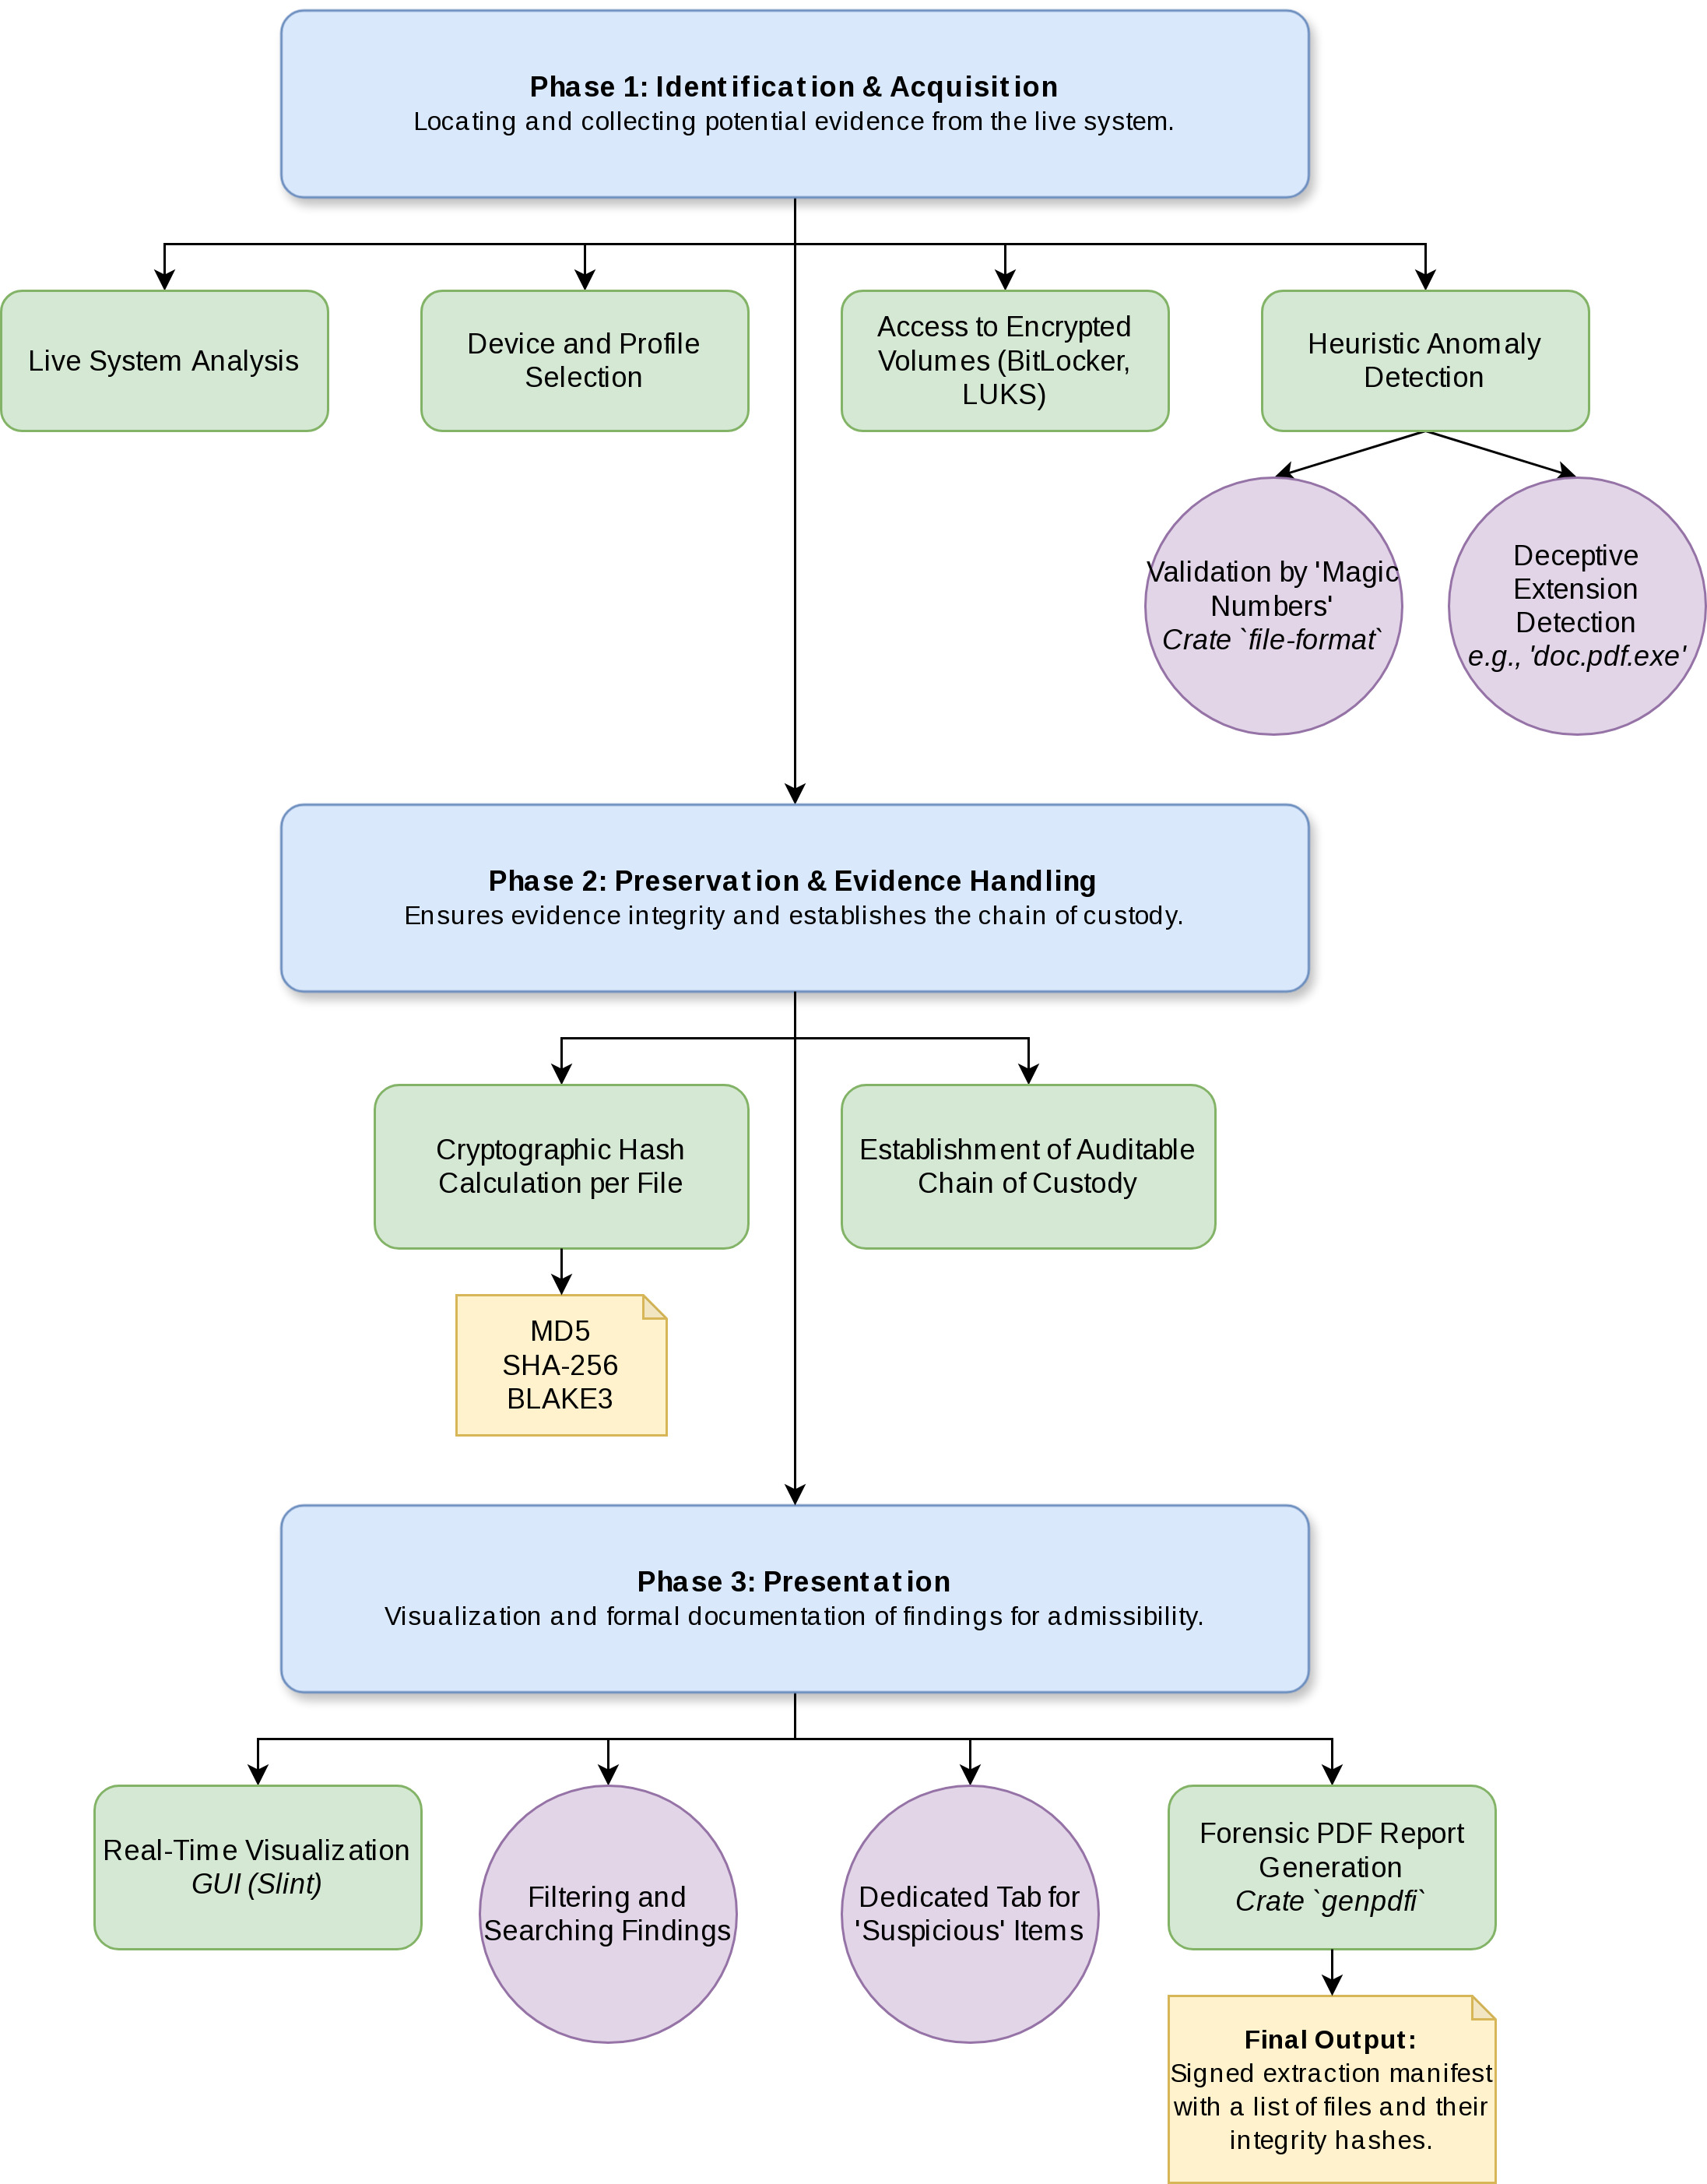
\includegraphics[width=0.8\textwidth]{resources/foruster_features.jpg}
    \caption{Diagrama de las características de Foruster, mostrando sus capas modulares}
    \label{fig:features}
\end{figure}

\section{Illustrative examples}

Para demostrar las funciones principales de Foruster, consideremos un escenario de respuesta a incidentes en un entorno corporativo. Un analista forense necesita investigar la estación de trabajo de un empleado bajo sospecha de haber extraído información confidencial a un dispositivo de almacenamiento externo, todo ello sin interrumpir las operaciones del sistema.

El analista ejecuta Foruster directamente en el sistema activo. La aplicación presenta inmediatamente una lista de los dispositivos de almacenamiento conectados, incluyendo el disco principal del sistema (C:$\backslash$) y una unidad USB que se acaba de conectar. El analista selecciona ambos dispositivos para el análisis. A continuación, la interfaz le permite configurar los perfiles de búsqueda. Dado que la sospecha es la exfiltración de datos, elige los perfiles predefinidos de "Documentos" e "Imágenes", que están configurados para buscar tipos MIME y extensiones de archivo comunes asociados a estos formatos.

Al iniciar el análisis, la interfaz muestra en tiempo real el progreso del escaneo, actualizando contadores de archivos analizados, coincidencias encontradas y, crucialmente, archivos sospechosos. Una vez finalizado el proceso, el analista navega a la pestaña de resultados "Sospechosos". Allí encuentra un archivo llamado informe\_anual.jpg ubicado en la unidad USB. Foruster lo ha marcado como sospechoso porque, aunque su extensión es .jpg, la validación de su contenido mediante "magic numbers" (realizada por el crate file-format) ha determinado que en realidad es un archivo comprimido (application/zip). Este hallazgo es de alta prioridad, ya que sugiere un intento de ofuscar datos confidenciales.

Finalmente, el analista utiliza la función de exportación para generar un informe forense en formato PDF. Este documento, creado por el crate genpdfi, no solo resume las estadísticas del análisis y los perfiles utilizados, sino que también incluye una sección detallada sobre los hallazgos sospechosos. En esta sección, se lista el archivo informe\_anual.jpg, el motivo de la sospecha (discrepancia entre extensión y contenido) y sus correspondientes hashes criptográficos (MD5, SHA-256 y BLAKE3), garantizando así una cadena de custodia auditable y preservando la integridad de la evidencia digital para su posterior análisis en profundidad.

{
\color{red}

Para complementar esta descripción textual, se ha preparado un breve vídeo de demostración (Screencast 1) que muestra este mismo proceso en acción, desde la selección del dispositivo hasta la generación del informe final. El vídeo está disponible como material suplementario junto a este artículo.
}

\section{Impact}
El principal impacto de Foruster reside en su capacidad para cambiar el paradigma del análisis forense digital, desplazándolo desde la investigación post-mortem de sistemas apagados hacia un análisis dinámico en sistemas vivos. Esta capacidad no solo mejora la eficiencia de las investigaciones existentes, sino que también abre nuevas vías de investigación y modifica la práctica diaria de los analistas forenses y equipos de respuesta a incidentes.

La disponibilidad de Foruster permite mejorar la búsqueda de respuestas a preguntas de investigación existentes sobre la volatilidad de la evidencia digital. Al operar en un sistema activo, el software permite capturar el estado de los archivos en un momento preciso, lo que facilita estudios comparativos entre la evidencia obtenida en vivo y la extraída de una imagen forense tradicional. Esto ayuda a cuantificar qué artefactos se pierden o alteran al apagar un sistema, un área de constante interés en la ciencia forense. Además, la herramienta agiliza la fase de triaje en una investigación, permitiendo a los analistas determinar rápidamente si un sistema justifica un análisis más profundo y la creación de una imagen completa, optimizando así el uso de tiempo y recursos.

Asimismo, la existencia de Foruster plantea nuevas preguntas de investigación que pueden ser exploradas. Por ejemplo, ¿cuál es el impacto en el rendimiento de un sistema anfitrión mientras se ejecuta un análisis concurrente con Foruster y cómo puede minimizarse para evitar la alteración de la evidencia? O, ¿pueden desarrollarse heurísticas de detección de anomalías en tiempo real más sofisticadas, basadas no solo en metadatos sino también en el comportamiento de los archivos? El uso de Rust como lenguaje de desarrollo también abre una línea de investigación sobre cómo las garantías de seguridad de memoria influyen en la fiabilidad y la solidez forense de las herramientas de software.

En términos de la práctica diaria, Foruster introduce un cambio fundamental en el flujo de trabajo de un analista. En lugar de que el primer paso sea desconectar el equipo, ahora es posible realizar un escaneo preliminar no invasivo. Esta capacidad es especialmente transformadora cuando se trata de volúmenes cifrados, ya que Foruster opera sobre el sistema de archivos descifrado y montado, eludiendo la necesidad de procesos complejos de descifrado offline y permitiendo el acceso inmediato a los datos.

Dado que Foruster es un proyecto de reciente creación, su uso aún no está extendido. Sin embargo, al ser una herramienta de código abierto y multiplataforma, alojada en un repositorio público de GitHub, está disponible para su adopción por parte de analistas forenses, investigadores académicos y profesionales de la ciberseguridad. La publicación de este artículo busca fomentar la creación de una comunidad de usuarios y contribuidores que impulse su difusión. Actualmente, no se conoce su uso en entornos comerciales ni ha dado lugar a la creación de empresas derivadas, pero su licencia de código abierto (GPLv3) permite su evaluación e integración en servicios de consultoría de seguridad o respuesta a incidentes.

\section{Conclusions}

\section*{Acknowledgements}
\label{}
Esta iniciativa se realiza en el marco de los fondos del Plan de Recuperación, Transformación y Resiliencia, financiados por la Unión Europea (Next Generation) - Instituto Nacional de Ciberseguridad (INCIBE) en el proyecto C108/23 “Detección de Falsificación de Documentos de Identidad mediante Técnicas de Visión por Computador e Inteligencia Artificial”.


%% The Appendices part is started with the command \appendix;
%% appendix sections are then done as normal sections
%% \appendix

%% \section{}
%% \label{}

%% References:
%% If you have bibdatabase file and want bibtex to generate the
%% bibitems, please use
%%
%%  \bibliographystyle{elsarticle-num}
%%  \bibliography{<your bibdatabase>}

%% else use the following coding to input the bibitems directly in the
%% TeX file.

\begin{thebibliography}{00}

%% \bibitem{label}
%% Text of bibliographic item

\end{thebibliography}

\end{document}
\endinput
%%
%% End of file `SoftwareX_article_template.tex'.

%%% Local Variables:
%%% mode: latex
%%% TeX-master: t
%%% End:
